%%==================================================
%% chapter01.tex for BIT Master Thesis
%% modified by yang yating
%% version: 0.1
%% last update: Dec 25th, 2016

%% modified by Meng Chao
%% version: 0.2
%% last update: May 29th, 2017
%%==================================================
\chapter{绪论}
\label{chap:intro}

\section{论文研究目的与意义}
近年来微小型无人机发展日趋迅速,对无人机导航系统的要求逐步提高,现有的经典导航方法在一些场景中受到限制。例如, GPS 只能用于开阔无遮挡的室外环境,且定位精度不高(非差分)。高精度的惯导系统成本过高难以民用,低成本IMU精度较差,且惯导系统只能估计无人机自身状态,无法感知周围的环境信息。无线信号定位方法需要预先布置使用场景,难以大范围应用。基于机器视觉的定位算法因其硬件成本低廉,精度较高,可感知丰富的环境信息,无需事先布置场景等优势,成为目前无人机定位导航的研究热点。

对于视觉定位而言一个基本而重要的问题是如何通过二维的图像信息分析景物的三维结构,确定相机在其中的位置\upcite{[1.1]}。经过近30年的长足发展,人们在这个问题上取得了众多令人兴奋的成果,这其中离不开一项基本技术的研究:同步定位与地图重建(Simultaneous Localization and Mapping,SLAM),特别是基于视觉的SLAM技术。同步定位与地图构建技术(下文简称SLAM),旨在解决携带传感器的运动物体,在运动过程中如何对自身进行定位,同时以合适的方式建模周围环境的问题\upcite{[1.2]}。根据所携传感器的不同,可以把 SLAM分成激光和视觉两大类。激光SLAM在理论和实践上均较为成熟,已较好地应用于机器人等行业。而视觉SLAM则起步较晚,如果把环境限定在光照、纹理充足,由静态的刚体组成的场合,现有的视觉SLAM可以令人满意地运行。而针对实际应用场景,无论从精度、效率、鲁棒性上来说,都与理想的情况相去甚远。

在视觉SLAM算法中,根据所用传感器不同可以分为RGB-D SLAM,双目SLAM和单目SLAM三种\upcite{[1.3]}。无人机一般运行在大场景和变尺度的环境下,而 RGB-D相机量程有限,噪声大;双目相机受到基线的限制,在景深远大于基线距离时获得的深度误差很大而退化成单目,都无法用于大尺度和变尺度场景中。而单目相机不存在基线与深度测量量程的限制,结构简单,计算效率高,广泛应用于大尺度环境和变尺度场景。

当前的单目SLAM算法很难在保证定位精度和鲁棒性的前提下提供丰富的环境地图;并且由于单目相机无法提供深度信息,得到的运动轨迹和环境地图的尺度不确定,因而无法用于导航和环境感知。本文研究并对比主流单目SLAM算法,对基于特征的单目SLAM算法进行改进,研究基于概率逆深度估计的单目半稠密SLAM算法,并将惯性测量单元(IMU)与单目进行信息融合。在保证定位精度和鲁棒性的前提下,得到有确定尺度的轨迹和环境半稠密地图,应用于无人机在陌生环境下的定位和导航。
\section{无人机定位技术研究现状}
随着多旋翼无人机的发展,其飞行范围从实验区域扩展到室外丛林,城市和室内生活区。但复杂环境中一般都在噪声干扰、信号遮挡和动态运动目标,这对无人机的导航定位提出了更高的要求。传统的导航定位方法如GPS和惯导系统存在局限,如GPS只能用于室外且对于非差分的GPS定位精度较低。低成本惯导本身存在较大漂移,定位精度差。近年来利用机载传感器(如激光雷达、摄像头或光流等)进行多传感器数据融合逐渐成为无人机定位与导航领域的研究重点。

美国犹他州立大学\upcite{[1.4]}的四旋翼无人机采用Gumstix的Verdex Pro XL6P芯片,机载传感器为惯性测量元件(IMU)、声纳传感器,单目摄像头,红外探测摄像头等。采用基于视觉图像的SLAM算法进行无人机定位和导航,实现在地面站平台,导航信息通过无线数传发送给无人机,完成无人机的导航和任务规划,还可根据红外探测摄像头对室内物体进行检测。宾夕法尼亚大学\upcite{[1.5]}选用Ascending Tech-nologies GmbH无人机,使用Intel Atom 1.6 GHz CPU作为控制平台,机上携带激光雷达,摄像机、IMU和两个测高望远镜,采用基于网络搜索的ICP算法利用激光雷达进行定位,利用视觉SLAM矫正位姿误差,并利用扩展卡尔曼滤波(EKF)实现多传感器数据融合。依靠多层次的环境重构、定位、轨迹规划和控制在室内实现全自主飞行,并且对外部环境的变化具有较好的鲁棒性。弗莱堡大学\upcite{[1.6]}选用Mikrokopter无人机,机上载荷包括激光雷达和航姿系统,采用激光SLAM算法并通过粒子滤波实现多传感器融合,完成在已知或位置环境下的见图与定位、航迹规划和无人机控制。

综上所述,SLAM技术已广泛应用于无人机定位与导航。相比于传统的惯性导航和卫星导航,SLAM技术不受限于室内外场景,定位精度高,结构简单,漂移小,功耗低,鲁棒性好,不需要环境的先验信息,可以满足多旋翼无人机的定位和导航需要。

\section{视觉SLAM国内外研究现状}
\subsection{国外研究现状}
SLAM技术最早始于1985年\upcite{[1.7]},在1986年至1990年期间,R.Smith提出了SLAM问题并给出了初步的解决方案\upcite{[1.8]}。他率先以概率形式讨论机器人轨迹与地图之间的不确定性,并将扩展卡尔曼滤波应用在SLAM问题。相比于之前的确定性方法,基于概率形式的方法更灵活、搞笑的表达轨迹与地图的估计,可以在理论上分析、推导SLAM问题的数学表达。这一方法在随后的十几年间成为主流,得到了充分的研究和扩展\upcite{[1.9],[1.10]}。主要的研究方向包括:扩展EKF应用场景的规模\upcite{[1.11],[1.12]}、解决EKF中的数据关联问题\upcite{[1.13]}、减少EKF的计算量\upcite{[1.14]}、使用其他种类的滤波器\upcite{[1.15],[1.16]}。

遵循前辈们的轨迹,研究者们在21世纪初期开始了视觉SLAM的研究。与激光传感器不同,视觉传感器的运动天生属于三维空间。不过,图像跟踪的特征点可以看做SLAM的路标点,适用于传统SLAM算法的位姿——路标框架\upcite{[1.17]}。相比于传统的激光SLAM算法,视觉传感器具有便宜、轻便、信息丰富等多种优点,但是它的特征点数量多,没有距离信息,对算法和硬件设计提出了挑战。2007年,A.J.Davison经过长期的研究,首次实现实时视觉SLAM EKF SLAM系统——MonoSLAM\upcite{[1.2]}。这具有里程碑的意义,该系统以EKF作为后端,跟踪前端提取的很稀疏的Harris特征点\upcite{[1.18]},减少了计算规模,把视觉SLAM算法实时化。

21世纪中,视觉SLAM经历了以上一系列重要的发展,产生了一批现有的视觉SLAM解决方案,如表\ref{tab1.1}所示。SLAM技术的发展可以分理论和算法两个方面。

\begin{table}		%表格环境
% \multicolumn是跨列功能,第一个参数2,表示跨两列,第二个参数c|,表示文字置中,并在栏位右边画一条直线框,最后一个参数即是要填入的文字
%\multirow是跨行功能,第一个参数2,表示跨两行,第二个参数*,表示系统自动调整文字,最后一个参数即是要填入的文字
\newcommand{\tabincell}[2]{\begin{tabular}{@{}#1@{}}#2\end{tabular}}		%单元格内容强制换行
\renewcommand\arraystretch{1}		%增加行间距
\centering
\caption{现代代表性SLAM方案}   % 表格标题,在表格内容之前
\label{tab1.1}
	\begin{tabular*}{\textwidth}{@{\extracolsep{\fill}}cccc}  %生成行和列的表格
	\toprule
	方案名称 &发布时间 &传感器类型 &特点 \\
	\midrule
	MonoSLAM\upcite{[1.2]}		&2007		&单目		&第一个实时SLAM,EKF+稀疏角点		\\
	PTAM\upcite{[1.19]}			&2007 		&单目		&关键帧+BA,优化作为后端 			\\
	ORB-SLAM\upcite{[1.20]}		&2015		&单目为主		&ORB特征+三线程 					\\
	LSD-SLAM\upcite{[1.21]}		&2014		&单目为主 	&直接法+半稠密 					\\
	SVO\upcite{[1.22]}				&2014		&单目		&稀疏直接法,仅是视觉里程计 		\\
	DTAM\upcite{[1.23]}				&2011		&单目		&直接法,单目稠密重建,需GPU加速	\\
	DVO\upcite{[1.24]}				&2013		&RGB-D		&RGB-D直接法,稠密地图				\\
	DSO\upcite{[1.25]}				&2016		&单目		&单目直接法,当前效果最好的直接法	\\
	RTAB-MAP\upcite{[1.26]}			&2013		&双目/RGB-D	&较大场景的实用RGB-D SLAM			\\
	RGB-D-SLAM-V2\upcite{[1.27]} 		&2014		&RGB-D		&完整的RGB-D稠密建图				\\
	OKVIS\upcite{[1.28]}				&2015		&多目+IMU	&以优化融合为主的关键帧VIO			\\
	ROVIO\upcite{[1.29]}				&2015		&单目+IMU	&EKF为融合为主的VIO				\\
	Kinection Fusion\upcite{[1.30]} 	&2011		&RGB-D		&RGB-D在线重建经典工作				\\
	Elastic Fusion\upcite{[1.31]} 	&2015		&RGB-D		&RGB-D在线重建,效果较好			\\
	Cartographer\upcite{[1.32]}		&2016		&激光		&支持回环的激光SLAM				\\
	LOAM\upcite{[1.33]}				&2014		&激光		&当前效果最好的激光SLAM			\\
	\bottomrule
	\end{tabular*}
\end{table}

\subsubsection*{理论发展}
21世纪之后,视觉SLAM理论上的重要发展主要有两点:非线性优化方法的引入和矩阵稀疏性的应用。在视觉SLAM研究中,研究人员发现它和计算机视觉领域的Structure from Motion(SFM)很相似。SFM目的在于通过不同视角的相机重建整个场景的三维结构。它需要利用特征追踪以获得匹配点,然后利用非线性最小二乘构建Bundle Adjustment(BA)问题进行全局的优化,以获得精确的相机位姿和场景结构\upcite{[1.34]}。SFM与SLAM的主要差异在于,SFM本质上是离线算法,可以在数据采集完全后进行长时间的离线优化。SLAM必须实时运算。但SFM对BA问题的深入研究\upcite{[1.35]},对SLAM是有启发性的。特别是,对于传统的基于滤波器的SLAM算法,存在着一些局限性。

\begin{enumerate}[label={(\arabic*)}]
\item 首先,传感器的运动和观测不一定满足马尔可夫性。特别是当传感器的运动出现回环时,即运动到之前经过的地方,此时当前状态会受到之前状态的影响,而滤波器方法很难表示这种关联和约束。
\item EKF存在线性化误差和高斯分布假设带来的误差。EKF只在工作点处进行了一次近似(而不像优化方法在每次迭代时都进行线性近似),当工作点离最优状态较远时,会引入线性化误差。由于高斯分布在经过非线性函数后不再为高斯分布,此时再用高斯分布近似,亦会带来近似误差。
\item 在计算量和存储空间方面,EKF需要存储状态量的均值和协方差矩阵,复杂度为$\boldsymbol{O}(n^2)$,对于实际应用存在较大的限制。
\end{enumerate}

21世纪视觉现代SLAM的重要发展,是将主流的后端处理方式,从以EKF为代表的滤波器方法,发展为以非线性优化为主的优化方法,如图\ref{fig1.1}所示。假设状态和噪声满足高斯分布,EKF中的运动方程和观测方程相当于给定了各时刻状态变化的条件概率。从贝叶斯网络角度来看,对状态变量的最大后验估计(在先验位置时为最大似然估计),等同于在负对数情况下求误差的最小二乘\upcite{[1.36]}。相比于滤波器方法,非线性优化有几个明显好处
\begin{enumerate}[label={(\arabic*)}]
\item 可以处理更多的信息。滤波器方法必须假设马尔可夫性,将过去的状态边缘化,而优化方法可以考虑所有的运动和观测数据,使用了更多的信息。
\item 优化方法允许不断地迭代估计状态,对每个迭代点都在更新后状态处重新线性化,而EKF只进行一次。因此优化往往能求得更精确的解。
\item SLAM的优化问题可以自然地使用图模型或概率图描述,高效地处理回环检测。图模型的结构又能直接对应到BA问题中正规方程系数矩阵的稀疏结构,加速求解过程。
\end{enumerate}

如果将优化变量抽象成节点,把运动方程和观测方程引入的误差抽象成边,就能得到SLAM对应的一个图模型$\boldsymbol{G}=\lbrace \boldsymbol{V}, \boldsymbol{E} \rbrace$,称为图优化\upcite{[1.37]}。求解图模型就等同于求解SLAM问题。研究者们还开发了专用的图优化术因子图优化的工具\upcite{[1.37],[1.38]},被广泛地应用于当前的SLAM系统中。

\begin{figure}
    \centering
       	  \subfigure[]
       	  {
          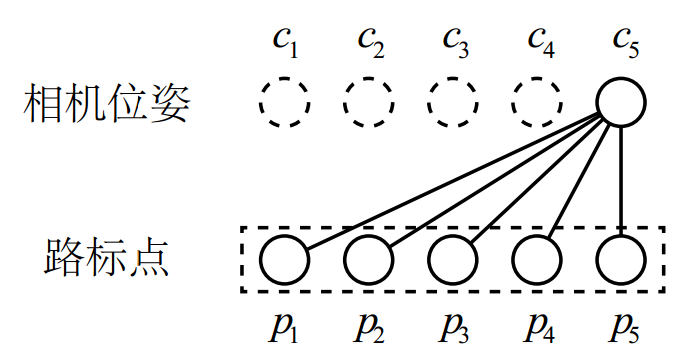
\includegraphics[scale=0.3]{figures/Fig1.1_a.png}          
          }                    
          \subfigure[]
       	  {
          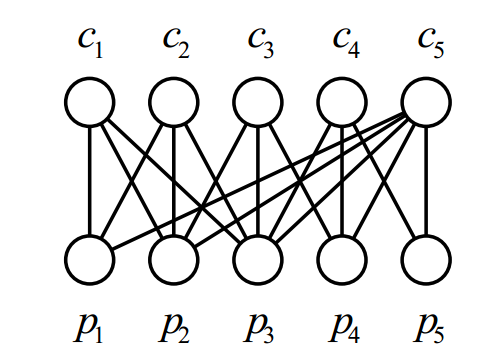
\includegraphics[scale=0.3]{figures/Fig1.1_b.png}
          }
     \caption{视觉SLAM理论发展}
\label{fig1.1}
\end{figure}


这些理论工具的引入,对SLAM系统的设计带来了很大改变。传统SLAM的主要任务是维护当前状态的估计,按照EKF理论对均值和方差进行预测——更新,将过去的状态边缘化到当前状态的协方差中。然而,随着非线性优化的流行,视觉SLAM的基本流程转向“抓取关键帧——非线性优化”的过程。通过在整个SLAM过程中定义一些具有重要意义的关键帧,就能够以它们为基本单位求解BA。这种行之有效的方法被称为基于关键帧的SLAM,是现在几乎所有视觉SLAM采用的方式。



\subsubsection*{算法发展}
SLAM理论上的发展促进了其算法框架的重要变化。首先,非线性优化可以处理更多的帧和地图点信息,使得SLAM开始分为“前端”和“后端”。前端主要负责实时的处理图像,提取路标点,抓取关键帧,关联传感器的观测值,初步估计运动状态和路标点位置,作为后端优化的初始值。而后端则通过非线性优化处理来端抽象的数据,求得更精确的轨迹和地图。这种区分前后端的方式,把计算繁重的任务放在了后台运行,同时亦能保证前端实时的响应。自从PTAM以来,这种做法开始成为SLAM的标准框架:前端被称为视觉里程计(VO)\upcite{[1.39]},后端则仍被称为后端或优化端。

前端和后端组成了基本SLAM结构,但是这样一个系统不具有丢失之后重新定位,或者重建用于导航、避障等用途的地图的能力。因此,完整的SLAM系统,通常在前后端之外,还具有回环检测和地图重建的能力。回环检测可以帮助SLAM消除VO中的累计误差,并且帮助SLAM在丢失之后重新进行定位\upcite{[1.40]}。建图模块则可建立与应用任务相关的地图,让SLAM更加实用\upcite{[1.41]}。


\subsection{国内研究现状}
相比于国外对视觉SLAM长时间的研究,国内研究人员对方向的认识多处于起步阶段。大部分研究工作都是零散的,系统、深入的工作则相对较少。不过,随着行业应用的兴起,该方向也正逐渐受到重视。华南理工梁明杰博士\upcite{[1.42]}、浙江大学的刘浩敏博士\upcite{[1.43]}、哈尔滨工程大学的权美香\upcite{[1.44]}等人都对视觉SLAM发展进行了整理。浙江大学章国锋教授的CAD实验室提出的RKSLAM\upcite{[1.45]}和RDSLAM\upcite{[1.46]},能够在移动端实现较好的定位效果。上海交通大学的邹丹平教授等人,提出了多相机同时进行的Co-SLAM\upcite{[1.47]},及基于线特征的StructSLAM\upcite{[1.48]}。香港科技大学沈劭劼教授\upcite{[1.49]}的小组,在关于飞行器SLAM和视觉惯导融合SLAM的方向上,包括视觉和惯导的标定、状态估计、初始化等问题,有着长足的研究。


以上,我们综述了SLAM在过去三十年间的发展。SLAM发展主要表现在为,理论方面从后端从EKF算法发展到非线性优化,并且认识到非线性优化中矩阵的稀疏性,保证算法实时性。算法层次,从维护当前状态的均值和协方差,变为对关键帧和地图点的维护与优化。应用角度,考虑后续导航和路径规划,构建半稠密或稠密的地图以提供丰富的环境信息;考虑算法鲁棒性,引入多传感器与视觉SLAM进行数据融合。

\section{论文主要内容和结构安排}
本文主要研究基于单目视觉的无人机同步定位与地图重建,针对单目SLAM应用于无人机导航中的一些关键技术进行研究和改进。本文首先建模分析多旋翼无人机的动力学模型,设飞行控制率并进行仿真验证,了解无人机的运动特性;对当前主流的单目SLAM算法进行对比分析研究,结合无人机运动特性选择合适的视觉SLAM算法;之后针对单目SLAM算法算法存在的问题进行改进,以更好的应用与无人机导航与定位。

第一章,主要介绍本文的研究背景、目的和意义,介绍无人机定位技术发展。综述同步定位与地图重建(SLAM)技术的发展和国内外研究现状,了解SLAM技术的发展方向和趋势。

第二章,针对本文的平台对象多旋翼无人机进行动力学建模,根据其动力学模型,采用经典控制理论设计PID控制率并进行仿真验证。了解多旋翼无人机飞行器的运动特性和定位和导航需求,便于研究和改进单目SLAM算法。

第三章,研究单目SLAM算法,详细介绍了SLAM算法的框架,理论原理。具体分析了当前两种主流的单目SLAM算法,基于特征的ORB-SLAM和基于直接法的LSD-SLAM,从定位精度、鲁棒性和地图重建效果三个方面进行比较。结合无人机的运动特性和导航需求,选择基于特征的ORB-SLAM算法作为无人机视觉定位和导航的解决方案,并提出ORB-SLAM算法存在的问题:重构地图稀疏和状态尺度不确定。

第四章,针对ORB-SLAM算法重构地图稀疏、环境信息少的问题,本章参考基于直接法的LSD-SLAM算法半稠密地图构建原理,研究基于特征的ORB-SLAM算法的半稠密重建。在原有算法的基础上,通过块匹配和一致性检验,在宽基线情况下重构半稠密地图,提供丰富的环境信息。

第五章,针对单目ORB-SLAM算法缺少尺度的问题,本章研究基于惯性测量单元(IMU)预积分的惯性-视觉SLAM算法。使用预积分算法对IMU数据进行处理,通过非线性优化将IMU预积分结果与视觉SLAM算法进行数据融合,获取环境的尺度信息并提高单目SLAM算法的鲁棒性。

总结与展望,对本文内容进行总结,并对未来工作进行展望。





\iffalse
\begin{figure}
  \centering
  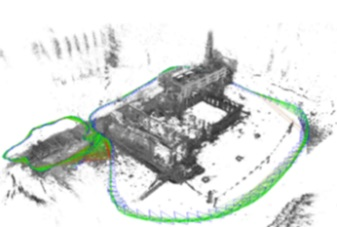
\includegraphics[height=0.5\textwidth]{figures/Fig1(1)}
  %\caption{The UAV equipped with an ASUS Xtion Pro Live RGB-D camera}
  %\label{Figure1.};
  
  \centering
  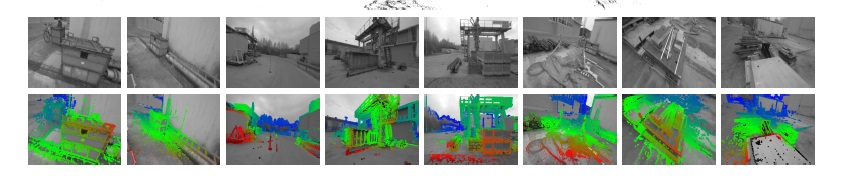
\includegraphics[width=0.75\textwidth]{figures/Fig1(2)}
  \caption{LSD-SLAM generates a consistent global map}
  %\label{referencename};
\end{figure}
\fi
